\documentclass[a4paper,11pt]{article}

\usepackage{amsmath}
\usepackage{amssymb}
\usepackage{amsfonts}
\usepackage[utf8]{inputenc} 
\usepackage[T1]{fontenc}
\usepackage{parskip}
\usepackage{graphicx}
\usepackage{epstopdf}
\usepackage[finnish]{babel}
\usepackage{csquotes}
\usepackage{subfigure}

\usepackage[backend=biber,style=numeric]{biblatex}
\addbibresource{viitteet.bib}

\begin{document}

{
\thispagestyle{empty}
{\large
Helsingin yliopisto
\par
MAT21022 - Johdatus valokuvan matematiikkaan
}

\vspace{7cm}

{\huge
Loppuprojekti:}
\par
{\Large \bf Kuvan kätkeminen toiseen kuvaan \\steganografian avulla}

\vspace{2cm}

{\Large Elli Kiiski}

\vfill

{\large \today}
}

\clearpage

\tableofcontents

\clearpage

\section{Johdanto}

\subsection{Steganografia}
Steganografia\footnote{Pahoittelut, tuli aika pitkä johdanto, mutta kun tämä vaan on varsin kiinnostava aihe!} on salauksen muoto, jossa kryptografiasta eroten pyritään piilottamaan varsinaisen informaation lisäksi myös se, että salasta informaatiota ylipäätään lähetetään. Tarkoituksena on siis piilottaa salainen viesti johonkin harmittomalta vaikuttavaan tiedon sekaan siten, ettei viestin mahdollinen kaappaaja tajua sen sisältävän mitään kaappaamisen arvoista.

Toisaalta siinä missä hyvää kryptografista salausta ei voi ulkopuolinen purkaa (ilman avainta) vaikka tietäisi toteutustavan täsmälleen, steganografisen salauksen toimivuus nojaa usein juurikin siihen, ettei ulkopuolinen tiedä salausmetodia. Tämän vuoksi salainen viesti kannattaa varmuuden vuoksi salata myös kryptografisesti, mikäli mahdollista.

Alkeellisimpia steganografian metodeja ovat esimerkiksi \enquote{näkymättömällä} musteella kirjoittaminen ja viestin kätkeminen pidemmän tekstin joukkoon. Historian ensimmäisenä steganografian käyttäjänä pidetään kreikkalaista Herodotusta, joka kirjoitti viestinsä luotetuimman orjansa päähän, ja lähetti tämän hiusten kasvettua takaisin viemään vastaanottajan luokse.

Nykypäivänä, kun lähes kaiken informaation välittäminen toimii digitaalisesti, voidaan steganografian avulla piilottaa tietoa paitsi kuviin ja teksteihin myös video- ja äänitiedostoihin. Tapoja totetuttaa steganografinen salaus digitaalisesti on olemassa lukuisia. Ensinnäkin moni fyysisistä menetelmistä, kuten viestin piilottaminen pidempään viestiin, voidaan toteuttaa yhtälailla. Sen lisäksi teknologia mahdollistaa täysin uudenlaisia keinoja, kuten tiedon piilottamisen musiikin äänentaajuuksiin tai valokuvan pikseleihin. Tutustutaan näistä jälkimmäiseen tarkemmin.

\subsection{Kuvan piilottaminen toiseen kuvaan}
\label{teoria}

Digitaaliseen kuvan pikseleihin on mahdollista kätkeä ihmissilmältä yllättävän paljon tietoa. Riippuen tietenkin kuvan koosta siihen on mahdollista piilottaa esimerkiksi kokonaisia kirjoja tai toisia valokuvia. Tarkastellaan seuraavaksi tarkemmpin kuvan piilottamista toiseen kuvaan LSB (least significant bit) -tekniikan avulla.

Tiedetään, että RGB-kuva koostuu pikseleistä ja kolmesta väritasosta. Täten sitä voidaan käsitellä kolmiulotteisena tietorakenteena, jonka jokainen arvo on luku väliltä 0-255. Nämä arvot voidaan puolestaan ilmaista kahdeksanbittisinä binäärilukuina, jotka sisältävät täsmälleen saman tiedon kuin aluperäinen pikselin arvo. Binäärimuotoisen esitystavan ansiosta on kuitenkin helpompi jakaa arvo osiin sen perusteella, mitkä bitit merkitsevät eniten ja mitkä vähemmän.

Tavallisessa binääriesityksessä merkitsevin (most significant) bitti on vasemmalla ja vähiten merkitsetvä (least significant) oikealla. Otetaan esimerkiksi luku $24$, joka on binäärinä $00011000$. Vertaillaan erotusta tähän alkuperäiseen lukuun, kun muutetaan joko ensimmäistä tai viimeistä bittiä:
\begin{itemize}
    \item $10011000=152$, erotus alkuperäiseen $152-24=128$
    \item $00011001=25$, erotus alkuperäiseen $25-24=1$
\end{itemize}
Yleistäen siis oikealta laskettuna $n$. bitin vaihtaminen muuttaa lukuarvoa $2^{n-1}$ verran.

Miten tätä havaintoa voidaan hyödyntää steganografiassa? On huomattu, ettei kuva oleellisesti muutu, vaikka pikseleiden arvot eivät ole täsmälleen alkuperäiset, kunhan muutos ole liian suuri. Näin ollen voimme käyttää muutamaa vähemmän merkityksellistä bittiä toisen viestin sisällön varastointiin ilman, että kuvassa tapahtuu havaittavia muutoksia.

Kun valokuvaan halutaan piilottaa toinen kuva, tehdään vastaavanlainen \enquote{biinääripilkkominen} kummallekin kuvalle ja piilotetaavan kuvan informaatio vaihdetaan piilopaikkana toimivan kuvan vähiten merkitsevien bittien arvojen tilalle. Tämän voi toteuttaa useammalla eri tavalla. Tapa kannattaa valita sen mukaan kuinka tärkeitä ovat mm. piilotettavan kuvan yksityiskohtien säilyttäminen ja salauksen huomaamattomuus paitsi paljaalle silmälle myös salauksia tunnistaville ohjelmille. Tässä työssä tarkastellaan LSB-menetelmistä muutamaa eri versiota.

\section{Ensimmäinen simppeli metodi}
\subsection{Lähtöasetelma}
Kuvitellaan seuraava tilanne: Elli on antanut ymmärtää opiskelevansa ahkerasti, vaikka oikeastaan elää parasta elämäänsä Matrixin vuosijuhlien jälkeisellä silliksellä. Äiti on kuitenkin epäileväinen ja pyytää kuvaa tilanteesta. Koska Elli ei tahdo suoranaisesti valehdella, hän päättää piilottaa todelliset puuhansa (kuva \ref{silliskuva}) aiemmin samalla viikolla ottamaansa kuvaan luennolta (kuva \ref{opiskelukuva}).

Kuvat on otettu kännykkäkameralla ja sittemmin rajattu kumpikin 560x560 pikselin kokoiseksi. Tiedostomuoto on jpg ja molemmat ovat värikuvia. Tässä tapauksessa ei haittaa, vaikka salaisesta kuvasta (kuva \ref{silliskuva}) menetetään merkityksettömimpien bittien tiedot, joten voidaan käyttää hyvin yksinkertaista menetelmää.

\begin{figure}
    \centering
    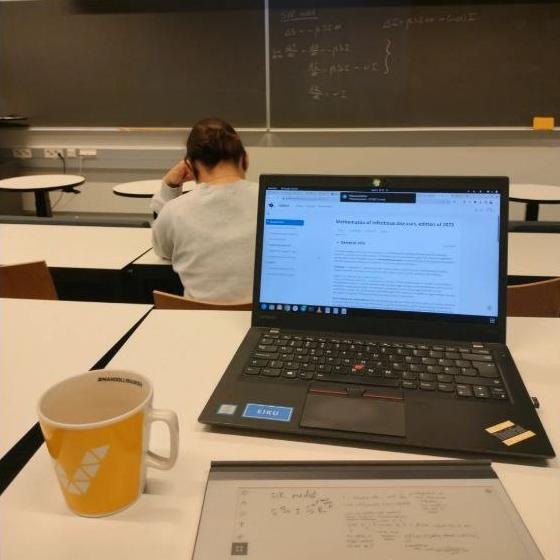
\includegraphics[width= 80mm]{kuvat/working-hard.jpg}
    \caption{Missä Elli muka on}
    \label{opiskelukuva}
\end{figure}
\begin{figure}
    \centering
    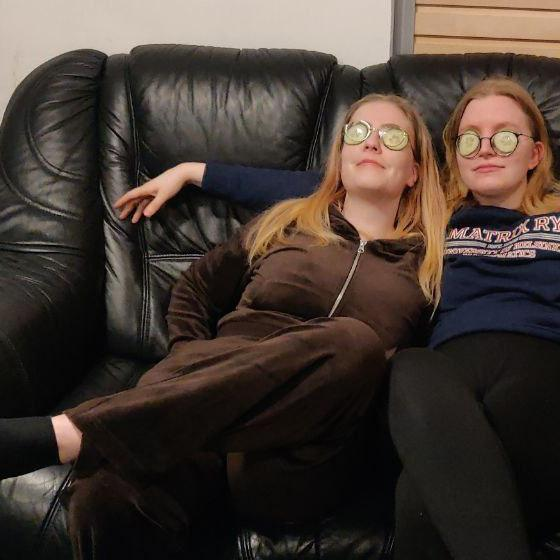
\includegraphics[width= 80mm]{kuvat/sillis-chilli.jpg}
    \caption{Ellin todellinen sijainti}
    \label{silliskuva}
\end{figure}

\subsection{Steganografisen metodin totetutus}

Toteutetaan MATLABilla simppeli funktio \texttt{simple\_encrypt}, joka ottaa parametreina piilona toimivan kuvan ja piilotettavan kuvan. Molemmat kuvat käydän värikerros kerrokselta ja pikseli pikseliltä läpi sekä pilkotaan kahteen osaan: neljään ensimmäiseen (merkitsevään) bittiin ja neljään viimeiseen (merkityksettömään) bittiin. Merkitsevät osat yhdistetään uudeksi arvoksi siten, että salaisen kuvan bitit liitetään piilokuvan bittien perään. Tämä arvo asetetaan uuden kuvan vastaavan pikselin arvoksi.

Mitä funktio siis käytännössä tekee, se korvaa kuvan merkityksettömän osan bitit toisen kuvan kuvan merkityksellisillä biteillä. Tätä on havainnollistettu kuvassa \ref{metodi1}. Teoriassa näin saadaan aikaan kuva, joka näyttää paljaalla silmällä alkuperäiseltä kuvalta, mutta sisältää samalla toisen kuvan, joka saadaan esiin vastaavalla salauksen purkufunktiolla.

\begin{figure}
    \centering
    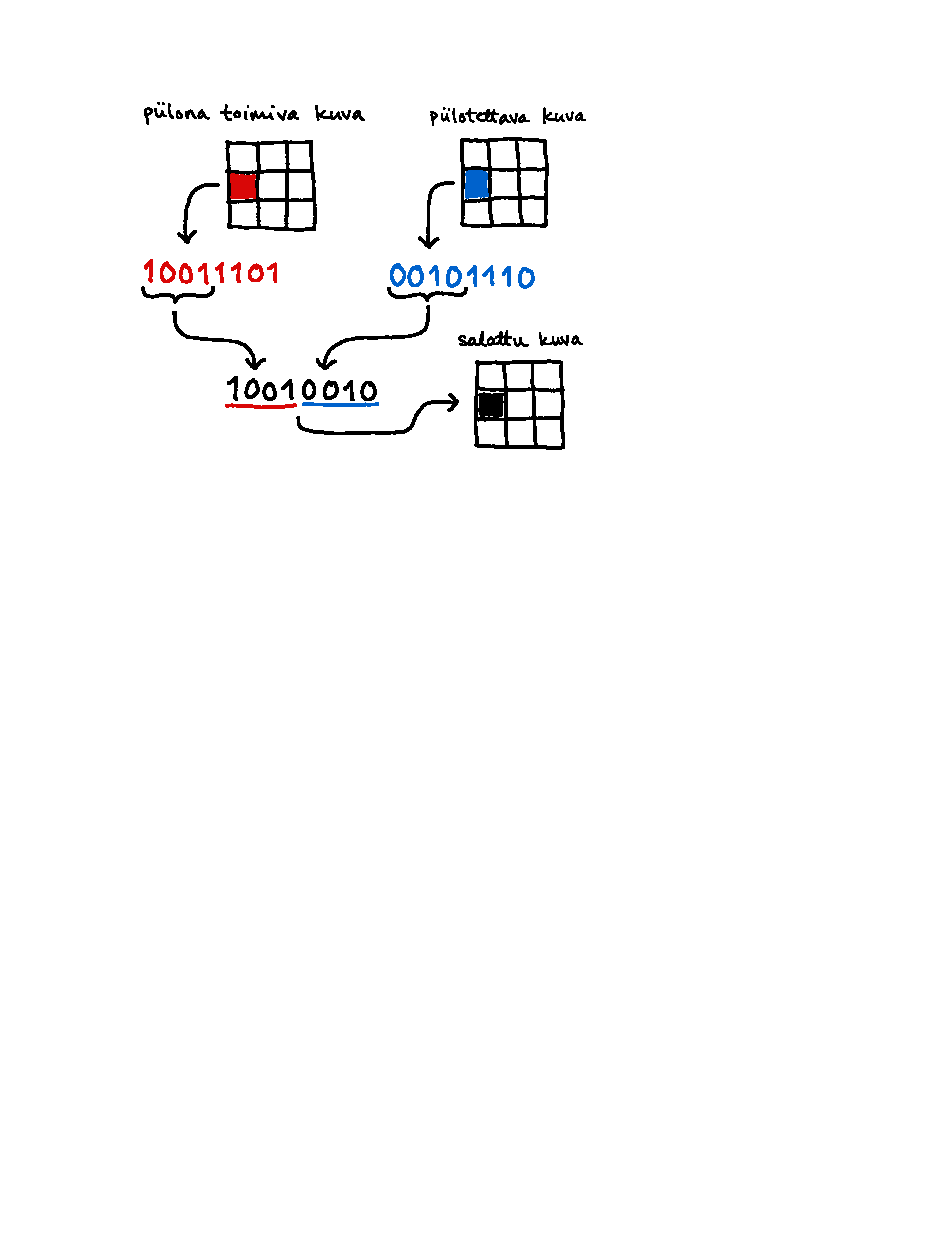
\includegraphics[width= 100mm]{kuvat/steganografia-esim1.pdf}
    \caption{Kuvan piilottaminen toiseen samankokoiseen kuvaan (kuvassa demonstroitu prosessi yhten väritason osalta)}
    \label{metodi1}
\end{figure}

Tällaisen salauksen purkamiseen on helppo toteuttaa funktio \texttt{simple\_decrypt}, joka ottaa parametrinaan salatun kuvan ja ikään kuin toimittaa samat askelet päinvastaisessa järjestykseeä. Tällä kertaa ollaan kiinnostuneita neljästä viimeisestä biteistä, jotka asetetaan puretun kuvan neljäksi ensimmäiseksi bitiksi. Koska neljän viimeisen bitin arvoa ei ole tallennettuna missään, voidaan ne yhtä hyvin asettaa kaikki nollaksi.

Teoriassa purettu kuva on nyt nähtävissä tarvittavan tarkasti samanlaisena kuin alkuperäinen. Kuvailtu salaus- ja purkumenetelmä kuitenkin hukkaa tiedon salattavan kuvan neljästä viimeisestä bitistä, mikä saattaa (osion \ref{teoria} tuloksen nojalla) aiheuttaa pahimmillaan $15$ suuruisen eron alkuperäiseen pikselin väriarvoon nähden. Vaikuttaako se liikaa? Entä huomaako salatusta kuvasta sen sisältävän toisen kuvan? Se selvitetään seuraavaksi.

\subsection{Tulokset}

Ajetaan salausfunktio \texttt{simple\_encrypt} kuvilla \ref{opiskelukuva} ja \ref{silliskuva} ja tarkastellaan sen tuottamaa salattua kuvaa (kuva \ref{salattu-simple}). Kuva näyttää toki ensivilkaisulta tavalliselta kuvalta luentopöydän äärestä, mutta tarkemmin katsottaessa siitä erottaa paitsi kummallisia \enquote{pikseliläikkiä} myös joitain yksityiskohtia salaisesta kuvasta. Toivottavasti äiti ei huomaa!

\begin{figure}
    \centering
    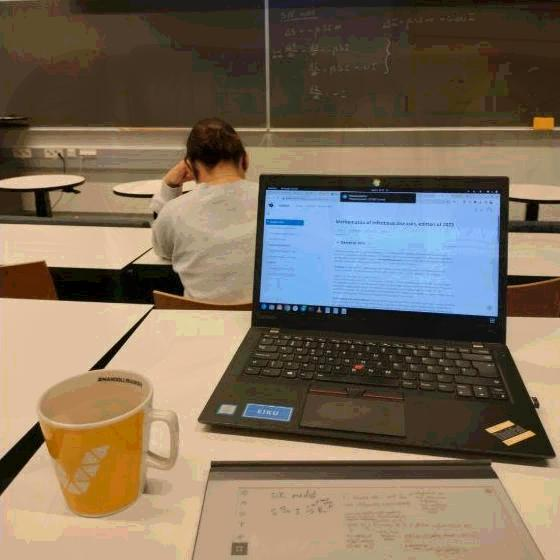
\includegraphics[width= 120mm]{kuvat/salattu1.jpg}
    \caption{Salausfunktiolla \texttt{simple\_encrypt} salattu kuva}
    \label{salattu-simple}
\end{figure}

Vaikuttaa siltä, että leikkausoperaatio neljännen bitin kohdalta oli liian raju, koska salatusta huomaa jopa ihmissilmällä epäjohdonmukaisuuksia ja vinkkejä salaisesta kuvasta. Jos käytettävissä on vieläpä alkuperäinen kuva, erotuksen ottamalla saa helposti varmistuksen, että jotain hämärää on tekeillä. Tutkimalla tätä erotuskuvaa (kuva \ref{erotus-simple1}), saadaan jo käsitys piilotetusta kuvasta ja voidaan epäilemättä suuremmitta vaivoitta arvata käytetty salausmetodikin.

\begin{figure}
    \centering
    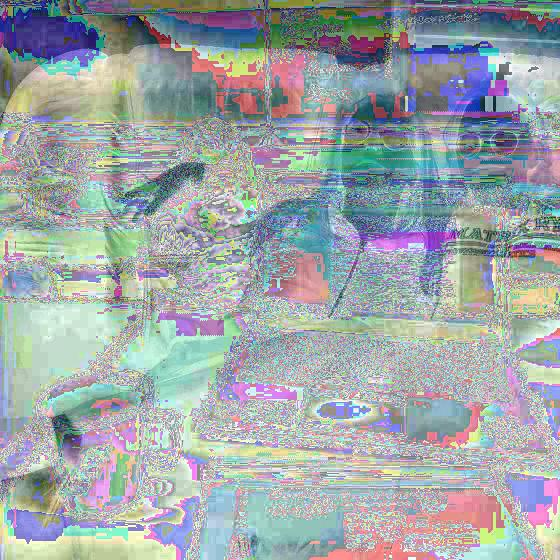
\includegraphics[width= 120mm]{kuvat/erotus1.jpg}
    \caption{Alkuperäisen kuvan \ref{opiskelukuva} ja salatun kuvan \ref{salattu-simple} erotus}
    \label{erotus-simple1}
\end{figure}

Kun salauus puretaan funktiolla \texttt{simple\_decrypt}, saadaan tuloksena oleellisilta osin alkuperäiseltä näyttävä kuva \ref{purettu-simple}. Kuvasta on erotettavissa tasavärisiä pikselialueita juurikin loppupään bittien puutteesta johtuen. Tapauksen kannalta oleellinen informaatio kuitenkin välittyy riittävän hyvin.

\begin{figure}
    \centering
    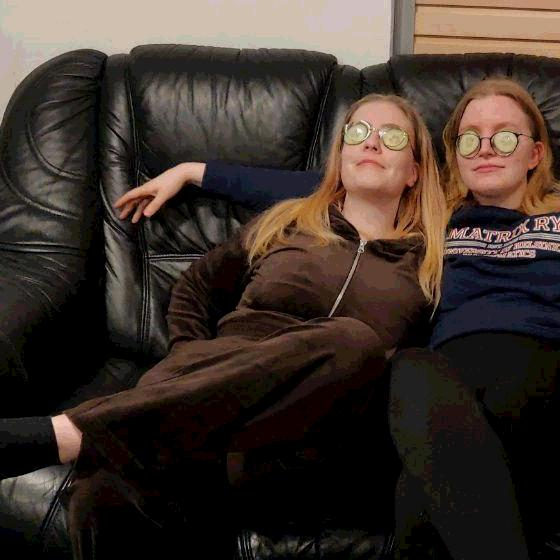
\includegraphics[width= 120mm]{kuvat/purettu1.jpg}
    \caption{Purettu kuvasta \ref{salattu-simple}}
    \label{purettu-simple}
\end{figure}

\subsection{Parannettavaa}

Simppelin metodin ongelmiksi havaittiin siis ensinnäkin sen epännistuminen salaisen kuvan peittämisessä ihmissilmältä. Toisekseen salattavan kuvan informaation säilyttämisessä on toivomisen varaa. Näitä molempia voidaan lähteä korjaamaan miettimällä uudestaan mistä kohdista pikselien binääriarvoja kannattaa alkaa pilkkomaan.

Kuvaa ei kovin helpoin keinoin\footnote{Ainakaan en keksi!!} sisällytettyä toiseen samankokoiseen kuvaan ilman, että jako jako täytyy tehdä bittijonon puolesta välistä. Tämä puolestaan aiheuttaa aiemmissa tuloksissakin nähdyt \enquote{pikseliläikät}, kun hienosäädöstä vastaavat merkityksettömimmät bitit uupuvat. Salatun kuvan elementtejä voidaan kuitenkin koittaa häivyttää sekottamalla bittien järjestystä, ennen niiden lisäämistä salattuun kuvaan (ks. osio \ref{sekoitus}).

Jos halutaan eroon \enquote{pikseliläikistä} tai säilyttää kaikki kuvan informaatio, tarvitaan naamioksi salattavaa kuvaa isompi kuva. Kun käytettävissä on enemmän pikseleitä, voidaan pienempi osa kustakin uhrata informaation säilyttämiseen tai vastaavasti sisällyttää kuvaan yhteensä isompi määrä toisen kuvan tietoa. Tai molemmat (ks. osio \ref{pieni-isoon}).

Yksi näin yksinkertaisen menetelmän huono puoli on myös se, että se on helppo arvata. Puhumattakaan steganografiaa tunnistavista ohjelmistoista, joille se olisi varmaankin maailman helpoin nakki. Tämän ongelman taklaaminen tosin vaatii vähän edityneempiä taktiikoita. Voimme kuitenkin koittaa parannella simppleitä funktioitamme hieman aiempien pohdintojen pohjalta.

\section{Paranneltuja metodeja lyhyesti}
\subsection{Bittien sekoittaminen}
\label{sekoitus}

Tavoitteena on korjata edellisen metodin ongelma, jonka vuoksi salatusta kuvasta oli nähtävissä linjoja salaisesta kuvasta sen tasaisissa kohdissa. Seuraava idea metodille ei kuitenkaan paranna lainkan pikselin arvojen säilymistä, joten \enquote{pikseläikistä} tuskin pääsemme eroon.

Kokeillaan tehdä muuten täysin samanlainen salausfunktio, mutta muuttaa salaisen kuvan merkitseviä bittejä jollakin logiikalla ennen niiden liittämistä toisen kuvan pikselin bittien perään. Bittien muuttaminen päinvastaisiksi eli binääriluvun komplementiksi on helppo laskutoimitus\footnote{En tosin saanutkaan helposti toteutettua tuota binäärilukujen vähennyslaskua MATLABILLA} ($1111-0101=1010$), joten testataan ensin auttaisiko se (funktio \texttt{complement\_encrypt}). 

Koska edellinen bittien sekoitustapa ei oleellisesi muuta viereisten pikseleiden arvoja toisiinsa nähden, vaan ainoastaan muuttaa isoimmat arvot pienimmiksi ja toisin päin, jää kuvaan näkyviin vielä ääriviivoja salaisesta kuvasta (kuva \ref{salattu-complement}). Mikä on ehkä yllättävämpää, tällä metodilla erotuskuvasta (kuva \ref{erotus-complement}) on vielä selkeämmin erotettavissa mikä kuva on yritetty salata. Metodi ei siis suinkaan ainakaan parantunut!

\begin{figure}
    \centering
    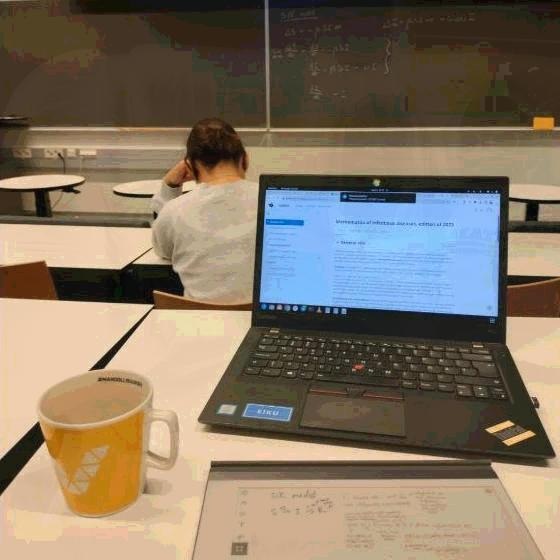
\includegraphics[width= 120mm]{kuvat/salattu2.jpg}
    \caption{Salattu ottamalla biteistä komplementti}
    \label{salattu-complement}
\end{figure}

\begin{figure}
    \centering
    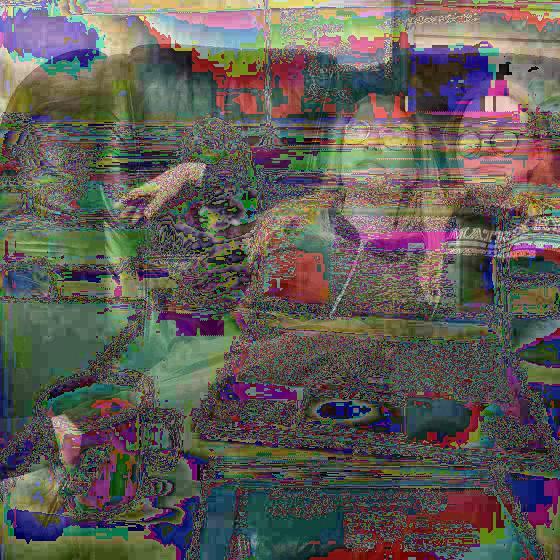
\includegraphics[width= 120mm]{kuvat/erotus2.jpg}
    \caption{Alkuperäisen kuvan \ref{opiskelukuva} ja komplementtisalatun kuvan \ref{salattu-complement} erotus}
    \label{erotus-complement}
\end{figure}

Bittien järjestyksen kääntäminen käänteiseksi voisi puolestaan oikeasti ratkaista käsillä olevan ongelman. Nimitäin tällöin jälleen loppuosaan merkityksettömistä biteistä tulee käänteisen bittijonon merkityksellisemmät, joten toisiaan lähellä olevat arvot (esim. $0100$ ja $0101$) muuttuvat toisistaan verrattain paljon eroaviksi ($0010$ ja $1010$). Tällä metodilla (\texttt{reverse\_encrypt}) saadaan kuin saadaankin kuva piilotettua paremmin toisen kuvan lomaan (kuva \ref{salattu-reverse}). Myös erotuskuvasta (kuva \ref{erotus-reverse}) huomataan, että pikseleisen arvot ovat paremmin sekaisin kuin aiemmin, vaikka tiettyjä ääriviivoja on toki vielä erotettavissa.

\begin{figure}
    \centering
    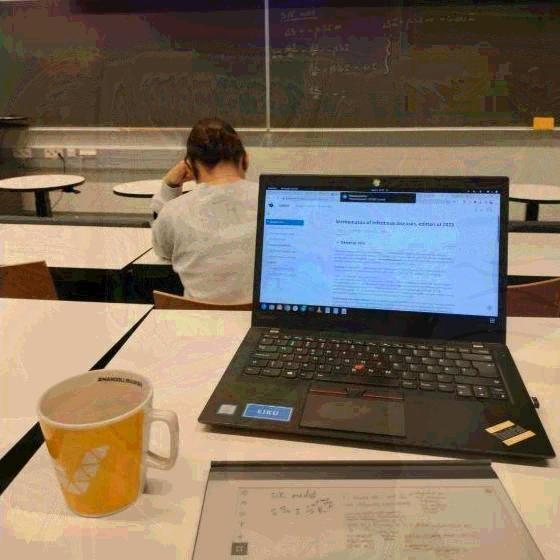
\includegraphics[width= 120mm]{kuvat/salattu3.jpg}
    \caption{Bittien järjestys kääntämällä salattu kuva}
    \label{salattu-reverse}
\end{figure}

\begin{figure}
    \centering
    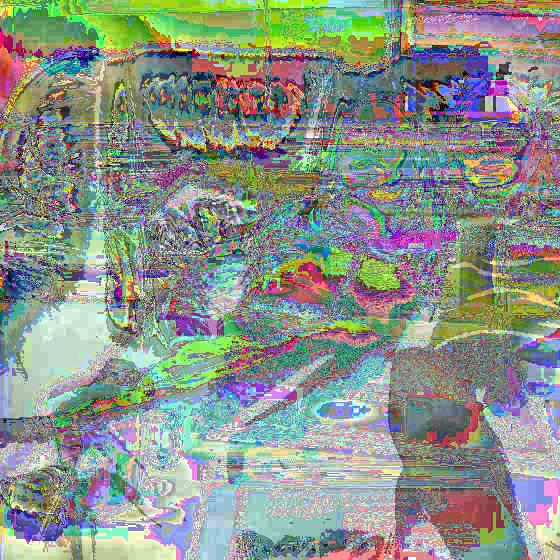
\includegraphics[width= 120mm]{kuvat/erotus3.jpg}
    \caption{Alkuperäisen kuvan \ref{opiskelukuva} ja bitit kääntämällä salatun kuvan \ref{salattu-reverse} erotus}
    \label{erotus-reverse}
\end{figure}

\subsection{Piilotus isompaan kuvaan}
\label{pieni-isoon}

Mikäli salaisesta kuvasta halutaan säilyttää kaikki informaatio, tarvitaan piilopaikaksi sitä isompi kuva. Isompaan kuvaan voidaan piilottaa informaatiota myös huomaamattomammin, kun säilömiseen voidaan käyttää esimerkiksi vain kahta viimeistä bittiä neljän viimeisen sijaan. Kuvassa \ref{metodi2} havainnollistetaan kuinka salaisen kuvan pikselien tarkat arvot saadaan piilotettua ja vieläpä aiempaa huomaamattomammin kuvaan, joka on neljä kertaa sen kokoinen.

\begin{figure}
    \centering
    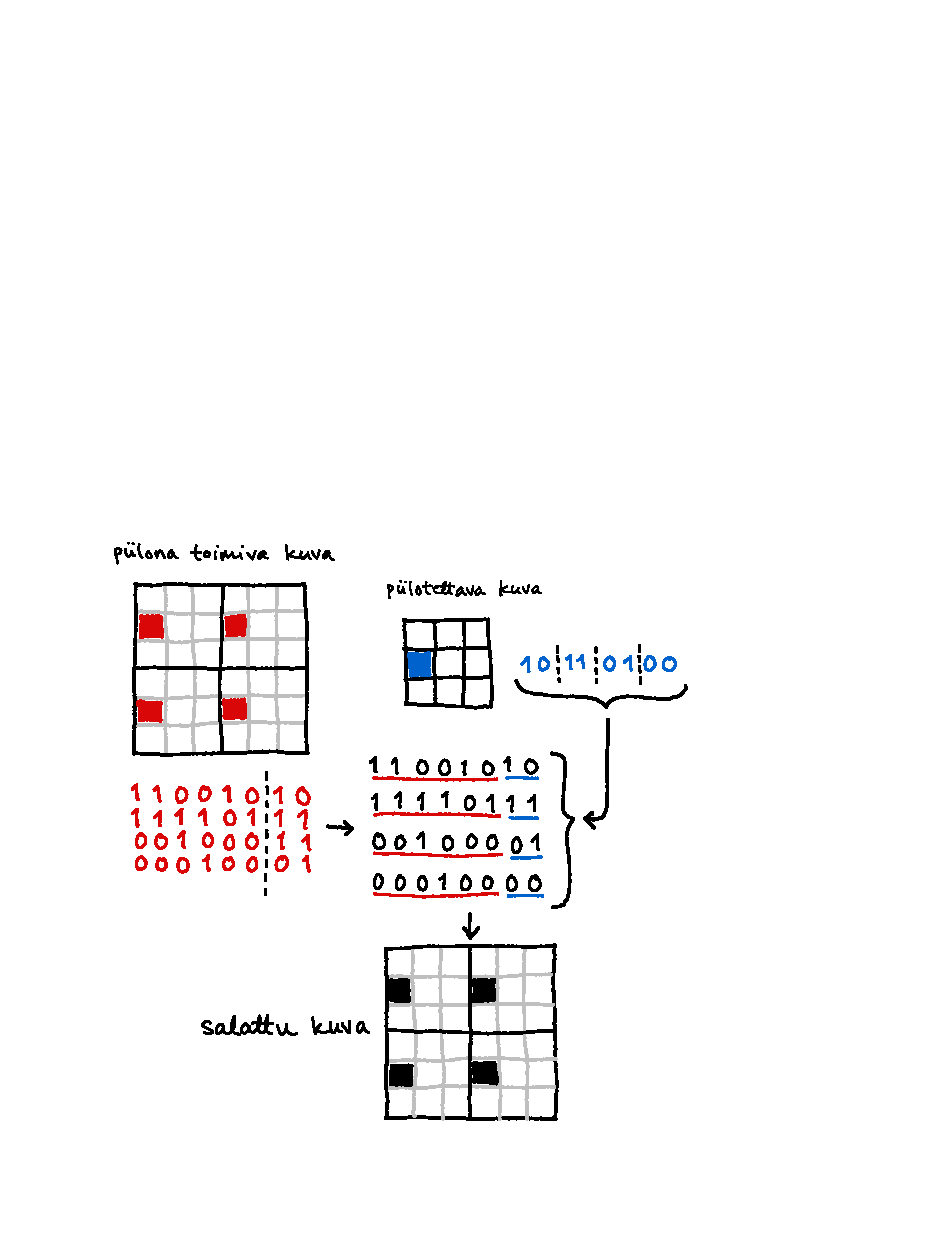
\includegraphics[width= 100mm]{kuvat/steganografia-esim2.pdf}
    \caption{Kuvan piilotus neljä kertaa itsensä kokoiseen kuvaan}
    \label{metodi2}
\end{figure}

Kyseisen funktion toteuttaminen ei ole paljoa aiemmin esiteltyjä metodeja kummoisempaa, ja se jää tämän projektityön ulkopuolelle. Odotettavissa olisi kuitenkin paljon huomaamattomampi salattu kuva sekä täysin alkuperäistä vastaava purettu kuva. Myös osion \ref{sekoitus} neuvoja voisi yhdistää tähän vieläkin paremman lopputuloksen saamiseksi.

\section{Johtopäätökset}

Tässä projektissa päästiin kokeilemaan yksinkertaisia steganografisia salausmenetelmiä. Toteutus onnistui varsin hyvin, vaikka aika ei riittänytkään metodien kehittämiseen kovin pitkälle. Kurssilla opitut taidot olivat hyvä pohja työn toteuttamiselle, vaikkakin esimerkiksi binäärilukujen käsittelyä MATLABilla piti opetella vielä sen lisäksi.

Oma mielenkiintoni aihetta kohtaa heräsi ja kasvoi melko suureksi, joten aion varmasti pelleillä näiden metodien kanssa myöhemmin vielä lisää. Salaisten viestien ujuttaminen ties minne kaikkialle kuulostaa hauskalta puuhailulta!

\nocite{*}
\printbibliography

\end{document}